\section{The Incremental Algorithm}
\label{sec:algo}
Intuitively, the incremental learning of a description from a large data source works
as follows. We first divide the data source into a sequence of smaller, manageable chunks.
For the first chunk, we learn a description $d_0$ using the format inference
algorithm described in section \ref{sec:review}. Then for each of the remaining chunks,
an {\em incremental learning step}, defined below, is performed.  

\begin{definition}[Incremental learning step]
Given an initial description $d$, and some new data $xs$, infer a new description $d'$ 
which is as similar to $d$ as possible such that $d'$ subsumes $d$ and describes $xs$.
\end{definition}

The new description $d'$ has to describe both the new data $xs$ and
all the old data which was described by $d$. 
In addition, we prefer $d'$ to be as similar to $d$ as possible because, first,
the learning process can begin with an initial description 
written by a human expert. 
Second, descriptions often serve as documentation of the data sources, and they are
read and modified by users from time to time. Keeping the documentation relatively stable increases
the ease of management. 

The rest of the section will focus on an algorithm that
performs one incremental learning step.
We first give the inductive definitions of
a description $D$, a data representation $R$, and an aggregate structure $A$. 
A description is an abstract syntax tree that includes a useful subset
of \pads{} features, and is what we want to learn. A data representation is 
the parse tree obtained from parsing some data using a description. 
An aggregate structure is the {\em accumulation} of parse trees, and it
includes data that cannot be parsed and therefore must be re-learned.

\begin{code}
\kw{Descriptions}:
Base ::= Pint | PstringME(re)
D ::=   
  Base             (Base token)
| Sync s           (Synchronizing token) 
| Pair (D1, D2)    (Pair)
| Union (D1, D2)   (Union)
| Array(D, s, t)   (Array)
| Option D         (Option)

\kw{Data representation}:
BaseR ::= Str s | Int i | Error
SyncR ::= Good | Fail | Recovered s 
R ::=
  BaseR
| SyncR
| PairR (R1, R2)
| Union1R R | Union2R R 
| ArrayR (R list, SyncR list, SyncR)
| OptionR R

\cdmath
\kw{Aggregation structure}:
A :: = 
  BaseA Base
| SyncA s
| PairA(A1, A2)
| UnionA($A_l$, $A_r$)
| ArrayA ($A_{elem}$, $A_{sep}$, $A_{term}$)
| OptionA A
| Opt A
| Learn [s]
\end{code}

In the above definitions, variable $re$ ranges over regular expressions,
$s$ and $t$ range over strings, and $i$ ranges over integers.
We assume just two types of base tokens: 
an integer token, and a string token that matches a
regular expression. Synchronizing tokens, or {\em sync tokens} for short, are constant strings. 
Synchronization tokens, such as white spaces or punctuations,
serve as delimiters in the data. Pairs and unions are self-explantory. 
A array has a element which is described by $D$, and a separator string $s$ and a
terminator string $t$. {\tt Option D} indicates $D$ is optional.

Parsing a base token can result in a string, an integer or an error.
On the other hand, parsing a sync token {\tt Sync s} can give three different results: 
{\tt Good}, meaning $s$ has been found at the beginning of the input, 
{\tt Fail}, meaning $s$ is not a substring in the current input, or 
{\tt Recovered s'}, meaning $s$ is not found at the current position in the input, but
can is {\em recovered} after ``skipping'' a string $s'$.
The parse of a pair is a pair of representations, and the
parse of a union is either the parse of the first branch, or the 
parse of the second branch. The parse of an array includes a list of parses for the element,
a list of parses for the separator and a parse for the terminator which appears at the end of
the array.

The aggregation structure ressembles the structure of the description $D$, 
with two additional nodes: an {\tt Opt} node, and a {\tt Learn} node. 
The {\tt Opt} node are always used above a {\tt BaseA} or a {\tt SyncA} node,
which indicates that the base token or the sync token underneath is missing in some of the parses
being aggregated, therefore, the token should be made optional.
Note the difference between {\tt Opt} nodes and {\tt OptionA} nodes. The latter 
just corresponds to the description {\tt Option D}. 
The {\tt Learn} node accumulates all the ``skipped'' data in the recovered mode. 
Such data is  ``unparsable'' and a sub-description needs be learned. The newly learned sub-descriptions 
will be added to the original description to get a new description. 
Essentially, the aggregate contains all the necessary information
to update the previous description.

\begin{figure}[t]
\begin{codebox}
incremental_step(d, xs) =
  as := [\kw{init_aggregate}(d)];
  foreach x in xs \{
    rs := \kw{parse}(d, x);
    as' := [];
    foreach r in rs \{
      foreach a in as \{
        a' := \kw{aggregate}(a, r); 
        as' := as' @ [a']
      \}
    \}
    as := as'
  \} 
  best_a := \kw{select_best}(as);
  d' = \kw{update_desc}(d, best_a);  
  return d'
\end{codebox}
\caption{Pseudo-code for the incremental learning step}
\label{fig:inc-learning}
\end{figure}

Figure \ref{fig:inc-learning} shows the overall algorithm for the incremental step in
pseudo-code. The {\tt init\_aggregate} function initializes an empty aggregate
structure according to a description $d$.  
Then for each data record $x$, we parse it into a list of parses $rs$
using the {\tt parse} function, which is essentially a {\em recursive descent parser}. 
We then call the {\tt aggregate} function to merge
each parse in $rs$ with each $a$ in the current list of aggregates. We use `@' to denote
concatenation of two lists. When we finish
parsing all the data lines and obtain a final list of aggregates $as$, we select
the best aggregate according to some criterion, and finally update the previous description
$d$ into $d'$ using the best aggregate. Next we use a couple of examples to
illustrate the parsing and the aggregation process which are key to this algorithm.

\begin{figure}[t]
\begin{center}
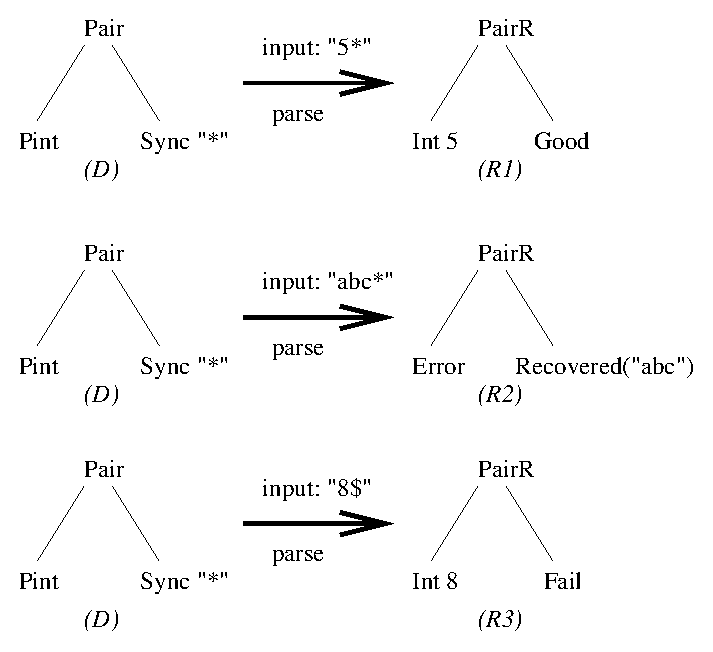
\epsfig{file=parse.eps, width=0.8\columnwidth}
\caption{Parse three input lines}\label{fig:parse}
\end{center}
\end{figure}

\begin{figure*}[t]
\begin{center}
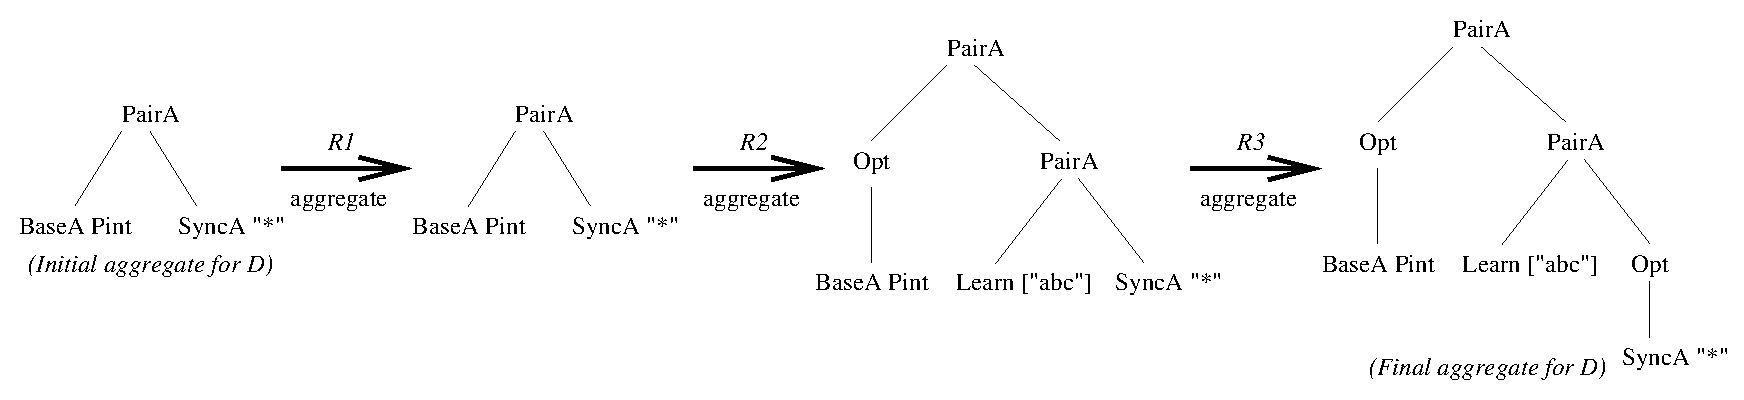
\epsfig{file=aggregate.eps, width=2\columnwidth}
\caption{Aggregate three parses into final aggregate structure}\label{fig:aggregate}
\end{center}
\end{figure*}

Suppose we have a description $d$, which is a pair of integer and a sync token ``*'',
and the the following new input data to be learned (in three lines):
{\small
\begin{verbatim}
5*
abc*
8$
\end{verbatim}
}

Figure \ref{fig:parse} shows the three data representations resulting from parsing the data lines,
and we call them $r_1$, $r_2$ and $r_3$, respectively. Notice that first line was parsed
without errors, second line contains an error for parsing {\tt Pint}, and some unparsable data
``{\tt abc}'', and the third line gives a {\tt Fail} node because the sync token was not found
at all. 
Figure \ref{fig:aggregate} shows the aggregation of $r_1$ through $r_3$ into an initially empty
aggregate structure. In general, {\tt Error} nodes and {\tt Fail} nodes in the parses causes the
creation of {\tt Opt} nodes in the aggregate. The unparsable data is collected in {\tt Learn} nodes
in the aggregate. 

Parsing a union involves attempting to parse the first branch and, if it has error, attempting
the second branch. This type of union semantics is known as the {\em deterministic choice}. 
When parsing an array, a {\em longest match} semantics is used, which means the parsing of
the array elements and separators will continue until no more progress can be made in
the input. We will not elaborate these semantics due to lack of space.


%\begin{codebox}
%parse_all (d, x) =
%  switch (d) \{
%    case Pint =>  
%      (s, remainder) := match_prefix(x, "[0-9+\-]+");
%      if s != "" then return (Int s, remainder)
%      else return [(Error, x)];
%    case PstringME(re) => 
%      (s, remainder) := match_prefix(x, re);
%      if s != "" then return (Str s, remainder)
%      else return [(Error, x)];
%    case Sync s => 
%      (s', prefix, remainder) := match(x, s);
%      if s' = s and prefix = "" then return (Good, remainder)
%      elseif s' = "" then return (Fail, remainder)
%      else return [(Recovered prefix, remainder)]
%    case (x:d1, d2) =>
%      rs1 := parse_all (d1, x);
%      rs2 := [];
%      foreach (r1, remainder) in rs1 \{
%        (r2, remainder2) := parse_all (d2, remainder);
%        rs2 := rs2 + [((r1, r2), remainder2)]
%      \}
%    case (d1 + d2) => 
%	parse_all(d1, x) @ parse_all(d2, x)
%    case d array(sep, term) =>
%  \} 
%\end{codebox}    
%

\cut{%%%%%%%%%%%%%%%%%%%%%%%%%%%%%%%%

The {\tt parse\_all} function takes a description $d$ and an input string $x$, and returns
a list of all possible parses along with their respective ending position in the input. 
This function implements a standard recursive descent parser which recursively matches the
description structure (and sub-structures) with the input. To parse a pair $x: d_1 * d_2$, 
we first call {\tt parse\_all} on $d_1$ and get a list of parses. 
And then for each of the parse $r_1$ and corresponding end position, we bind $x$ to $r_1$ in
a private environment and  parse $d_2$ to get parses $l_2$. 
Finally for each parse $r_2$ in $l_2$ and each parse $r_1$ in $l_1$, 
construct a representation $(r_1, r_2)$, and return a list of all such pairs.
To parse a union $d_1 + d_2$, we simply return the concatenation of list of parses from
parsing $d_1$ and the list of parses from parsing $d_2$. To parse $d~ array(s, t)$,
we repeatedly attemp to parse $d$ until there's no more progress in the input.
And in each iteration, we also add parses generated from parsing $t$ as well, as if
the array has been terminated at this iteration. Figure \ref{fig:parse_base}
shows the {\tt parse\_base} function which parses a base token. The {\tt match\_prefix}
function matches the prefix of an input string with a regular expression and returns
the matched string and the remainder in the input. The {\tt match} function looks for
the first match of $s$ in input $x$, and returns the matched string $s'$, the prefix string
in $x$ before $s'$, and the remainder in the input.

\begin{figure}[t]
\begin{codebox}
parse_base (b, x) =
  switch (b) \{
  case Pint => 
    (s, suffix) := match_prefix(x, "[0-0+\-]+");
    if s <> "" then return [(Int s, suffix)];
    else return [(Error, x)]
  case PstringME(re) => 
    (s, suffix) := match_prefix(x, re);
    if s <> "" then return [(Str s, suffix)];
    else return [(Error, x)];
  case Sync s => 
    (s', prefix, remainder) := match(x, s);
    if s' = s and prefix = "" then 
      return (Good, remainder)
    elseif s' = "" then 
      return (Fail, remainder)
    else return [(Recovered prefix, remainder)]
  \}
\end{codebox}
\caption{Function to parse a base token or a sync token} \label{fig:parse_base}
\end{figure}

As an example, let $d$ be {\tt (Pint, Sync "|") + (PstringME "[a-z]+", Sync "|")}, 
and $x$ be ``\verb#abc|#''. {\tt parse\_all(d, x)} gives the following two possible parses:
{\small
\begin{verbatim}
  inl (Error, Recovered "abc")
  inr (Str "abc", Good)
\end{verbatim}
}

The {\tt aggregate} function adds a parse into an existing aggregate structure. When there is
no errors in the parse, it makes no changes to the aggregate. If the parse contains 
an error or failure for parsing token $b$, then the aggregate component 
$b$ is transformed to $opt~ b$, to indicate that $b$ node is optional. 
If a parse contains a recovered data $Recovered~ r$, then
a optional learn node will be created before the sync node. And the new aggregate component will be
$(opt (l [r]),~ Sync~ s)$. If the aggregate structure already contains the learn node before this
sync node, then recovered data $r$ will be added to the list under $l$.

The {\tt select\_best} function computes a score by counting the total number of $opt$ and $l$ nodes
in each of the aggregates, and returns the one with the smallest number. The idea is that the
aggregate with the smallest number of added nodes is more likely to represent a new description
that is the closest to the original description. 

Finally, the {\tt update\_desc} function does two things. First, it invokes the format inference
algorithm to learn a sub-description for the data strings collected at each of the learn nodes
and replace the learn nodes with these new sub-descriptions. Then, it uses a number of rewriting
rules into improve the overall structure. We will discuss some of these rewriting rules in more
details in section \ref{sec:imp}.

}%%%%%%%%%%%%%%%%%%%%%%%%%%%%%%%%% END OF CUT %%%%%%%%%%%%%%%%

% - problem definition (as close to the previous description as possible) (but we don't
%   have a metric to measure how close yet, do we want to mention tree edit distance??)
% - overview of algorithm: parsing + aggregating + rewriting
% - parsing algo (parse rep, score metric, pseudo-code)
% - aggregating algo (in pseudo code)
% - selection of top aggregates
% - update original description
% - rewriting rules (data independent, data dependent, OptsTable)

